\documentclass[conference]{IEEEtran}
\IEEEoverridecommandlockouts
% The preceding line is only needed to identify funding in the first footnote. If that is unneeded, please comment it out.
\usepackage{cite}
\usepackage{amsmath,amssymb,amsfonts}
\usepackage{algorithm}
\usepackage{algorithmic}
\usepackage{graphicx}
\usepackage{adjustbox}
\usepackage{multirow}
\usepackage{textcomp}
\usepackage{xcolor}
\usepackage{hyperref}
\usepackage{tikz}
\usetikzlibrary{arrows.meta,positioning}

\begin{document}

% === TITLE ===
\title{SyncPilot: A Lightweight Initial-Calibration Scheduler for Asymmetric Multicore Pipeline Processing
}

% === AUTHOR ===
\author{
\IEEEauthorblockN{M. Hamdani Ilham Latjoro\IEEEauthorrefmark{1},
Adnan\IEEEauthorrefmark{1}}

\IEEEauthorblockA{\IEEEauthorrefmark{1}
Department of Informatics Engineering, Faculty of Engineering\\
Hasanuddin University, Makassar, Indonesia}

\IEEEauthorblockA{Emails:
latjoromhi25d@student.unhas.ac.id,
adnan@unhas.ac.id}
}
\maketitle

% === ABSTRACT ===
\begin{abstract}
Asymmetric Multicore Processors (AMP), which pair high-throughput Performance cores with power-efficient Efficient cores (e.g., ARM's big.LITTLE family), offer significant potential for edge Deep Neural Networks (DNNs), but standard OS schedulers often fail to exploit hardware heterogeneity. Prior dynamic schedulers address this but incur runtime overhead from continuous profiling. We propose SyncPilot, a lightweight pipeline framework built around Initial Calibration Runtime Cost Estimation (IC-RCE): each pipeline stage's cost is measured once during initialization, and this one-time calibration is what justifies keeping a static, hard-pinned Performance/Efficient worker-to-core mapping for the rest of execution, without further runtime measurement. On an ASUS GX10 (10$\times$ Cortex-X925 + 10$\times$ Cortex-A725), a 20-worker FSRCNN configuration reaches a 9.39$\times$ speedup over a serial baseline, with every configuration bit-exact against the ground truth. Benchmarked against unpinned Linux CFS, SyncPilot's static mapping is slightly outperformed by CFS's Energy Aware Scheduling (EAS) on an idle system. However, once background CPU noise pushes the Performance cluster into overutilization, EAS is disabled per Linux kernel policy and CFS's fallback balancer migrates heavy pipeline stages onto Efficient cores, inflating worst-case latency by 65.8\% (1067$\to$1769~ms); SyncPilot's mapping, structurally unaffected by this failure mode, limits the same growth to 21.9\% (1171$\to$1427~ms). We argue this static-versus-adaptive trade-off, not raw idle-system throughput, is the more representative measure of scheduler quality for non-idle, real-world edge deployments.
\end{abstract}

% === KEYWORDS ===
\begin{IEEEkeywords}
Asymmetric Multicore, Pipeline Parallelism, Runtime Cost Estimation, Heterogeneous Multicore, Energy Aware Scheduling, FSRCNN.
\end{IEEEkeywords}

% === I. INTRODUCTION ===
\section{Introduction}
The rapid evolution of edge computing has brought computationally intensive tasks, such as Deep Neural Network (DNN) inference, from cloud servers to local devices \cite{shi2016edge, zhou2019edge}. Modern edge hardware increasingly adopts Asymmetric Multicore Processors (AMP), notably the ARM big.LITTLE architecture, to balance high performance with energy efficiency \cite{greenhalgh2011biglittle, arm2013biglittle}. This architecture combines high-performance "Big" cores with power-saving "LITTLE" cores.

However, maximizing the potential of AMP for pipeline-parallel applications remains a challenge. The default Linux Completely Fair Scheduler (CFS) treats all cores generically, often failing to distinguish between compute-heavy and light tasks \cite{koufaty2010bias, vancraeynest2012pie}. This leads to suboptimal mapping, where heavy pipeline stages may be assigned to Efficient cores, creating bottlenecks, or light stages may unnecessarily occupy Performance cores, wasting energy.

Prior works have proposed dynamic scheduling solutions that monitor task execution times at runtime \cite{saez2010comprehensive}. While effective for adaptability, these methods introduce significant overhead due to continuous timing measurements and context switching, which is detrimental for real-time video processing applications. Conversely, static mapping approaches lack the flexibility to handle dynamic workloads \cite{wang2020pipeit}.

In this paper, we propose SyncPilot, a novel scheduling framework that bridges the gap between static efficiency and dynamic adaptability. Our core contribution is the Initial Calibration Runtime Cost Estimation (IC-RCE) mechanism. Instead of continuous profiling, SyncPilot performs a one-time calibration during the first task execution to estimate the computational cost of each pipeline stage. This calibration confirms that per-stage costs are stable and strongly skewed toward the final layers (Section~\ref{sec:layerprofile}), which is what justifies relying on a static, hardware-topology-based Performance/Efficient core pinning \cite{man7pthreadaffinity} for the remainder of execution instead of a continuously-monitored mapping.

The main contributions of this paper are summarized as follows:
\begin{itemize}
\item We propose IC-RCE, a lightweight one-time calibration mechanism that measures per-stage cost during the first task and eliminates the need for continuous runtime profiling thereafter.
\item We design a pull-based worker pool in which every thread autonomously selects work from a shared, priority-ordered stage queue (deepest-stage-first) without a central dispatcher, avoiding global-lock contention; the framework additionally supports an optional cost-threshold-gated pulling mode for explicit per-stage Performance/Efficient routing, which we describe in Section~\ref{sec:capacityaware} but leave to future evaluation on this platform.
\item We evaluate configurations on ASUS GX10 using FSRCNN, demonstrating that the 20-worker setup achieves the best throughput (9.39$\times$ speedup over the serial baseline) with numerically identical outputs across all configurations, and we show that SyncPilot's hard-pinned mapping is substantially more robust to system noise than an unpinned CFS/EAS baseline, at the cost of a modest idle-system throughput deficit.
\end{itemize}

% === II. RELATED WORK ===
\section{Related Work}

Research on scheduling for AMP has evolved from static partitioning to dynamic load balancing. The work closest to ours is Annisa et al. \cite{annisa2025fsrcnn}, which we build on directly and, unlike SyncPilot, uses a fixed OpenMP thread-per-stage mapping without a one-time cost calibration; the key differences are detailed at the end of this section. Annisa et al. \cite{annisa2025fsrcnn} investigated the transition from serial to parallel FSRCNN execution on an Orange Pi 5 using OpenMP with explicit CPU affinity. Their analysis showed that the heterogeneous big.LITTLE topology on that platform can benefit from broader worker scaling, with the strongest gains occurring when the workload is distributed across both the Big and LITTLE cores rather than being restricted to the fastest cores only. The key finding was that the stronger LITTLE cores reduce the severity of the straggler effect, making additional worker parallelism viable for this workload. Their analysis also confirmed that layer 8 (deconvolution) remains the primary computational bottleneck across all configurations, exhibiting the lowest speedup due to memory dependencies and potential race conditions when multiple threads access adjacent pixel regions without proper synchronization.

Wang et al. \cite{wang2020pipeit} proposed Pipe-it, a static partitioning method for CNN inference that relies on offline profiling to map layers to cores. While effective, it lacks runtime adaptability. AsyMo \cite{wang2021asymo} introduced offline planning for mobile CPUs but requires prior knowledge of the model structure. Recent works like DynPipe \cite{yuan2025dynpipe} utilize machine learning for dynamic adjustment but incur computational overhead during inference. Chronaki et al. \cite{chronaki2017task} propose dynamic and static scheduling policies for task-parallel programs on asymmetric multi-core systems based on critical-path detection and locality-aware task assignment; unlike SyncPilot, their approach targets general task-dependency graphs rather than the fixed, stage-structured pipeline mapping problem addressed here.

Unlike the OpenMP-based approach in \cite{annisa2025fsrcnn}, which assigns a fixed thread-per-stage mapping, SyncPilot introduces a pull-based worker pool that decouples threads from stages. The ASUS GX10 results indicate that the stronger Cortex-A725 cores reduce the performance gap that previously caused the straggler problem on more heterogeneous platforms. SyncPilot builds upon this finding with IC-RCE, a one-time calibration that eliminates continuous runtime profiling, and a static, hardware-topology-based Performance/Efficient core mapping whose fixed nature is what keeps it structurally immune to the OS-scheduler migration failure mode analyzed in Section~\ref{sec:noise}. Furthermore, advanced frameworks such as QLSA-MOEAD \cite{saad2026qlsa} utilize reinforcement learning for heterogeneous scheduling but are designed for cloud-scale DAG tasks, making them too heavy for embedded pipeline processing.

% === III. SYSTEM ARCHITECTURE ===
\section{System Architecture}
SyncPilot is designed around a centralized Worker Pool model. The architecture consists of four main components: the Pipeline Engine, the IC-RCE Module, the Asymmetry-Aware Core Mapper, and the priority-ordered Worker Pool itself.

\subsection{Pipeline Engine}
SyncPilot adopts a centralized Pull-Based Worker Pool model. Unlike traditional pipeline architectures that assign a dedicated thread to each stage (thread-per-stage), our model decouples threads from stages. 
The system consists of three primary components: (1) Shared Stage Queues that hold pending tasks for each pipeline stage, (2) A Worker Pool comprising threads pinned to specific core types, and (3) A Reorder Buffer to ensure output order preservation.
A key advantage of this model is the elimination of a central dispatcher. Instead of a manager pushing tasks to workers, each worker thread autonomously pulls tasks from the shared queues. This pull-based mechanism naturally balances the load, as idle workers proactively seek available tasks, minimizing idle time.

\subsection{Initial Calibration Runtime Cost Estimation (IC-RCE)}
The core novelty of SyncPilot lies in its IC-RCE mechanism. During the processing of the first task (Task ID 0), the framework measures the execution time of each stage using high-precision timers (\texttt{clock\_gettime}). These measurements are stored in a Cost Table (empirically reported in Section~\ref{sec:layerprofile}). Once all stages are processed, the system enters the "Steady State," where no further timing measurements are taken. This effectively reduces the profiling overhead to zero during the processing of subsequent tasks (Task ID $> 0$). In the configuration evaluated in this paper, the Cost Table serves as a validation instrument: it confirms that per-stage cost is stable across the run and heavily skewed toward the deconvolution stage, which is the empirical justification for relying on a \emph{static} core mapping (Section~\ref{sec:asymmap}) rather than a continuously re-evaluated one. SyncPilot's implementation also supports an optional mode, described in Section~\ref{sec:capacityaware}, in which the Cost Table is additionally consulted at task-pull time to gate which stages a Performance or Efficient worker may pick up; we did not enable this mode for the GX10 results reported here (Section~\ref{sec:limitations}).

\subsection{Asymmetry-Aware Core Mapping}
\label{sec:asymmap}
Upon initialization, and before any task is processed, each worker thread is pinned to a specific CPU core via \texttt{pthread\_setaffinity\_np}. SyncPilot detects Performance and Efficient cores automatically from \texttt{cpufreq/cpuinfo\_max\_freq} (the highest-frequency cluster is treated as Performance, the remainder as Efficient), or accepts an explicit core-ID list; workers are then assigned round-robin within each class, so that, e.g., a 20-worker run on a 10+10 topology pins the first 10 workers to Performance cores and the remaining 10 to Efficient cores. This mapping is fixed for the lifetime of the run: it does not change in response to which stage a worker happens to be executing, nor does it consult the IC-RCE Cost Table. Its role is purely topological — ensuring every worker has a dedicated, known-capability core — while the actual work-to-core matching emerges indirectly, since Performance-core workers execute the same priority-ordered pull loop faster than Efficient-core workers and therefore drain more tasks from the shared queues per unit time.

\subsection{Capacity-Aware Worker Pool}
\label{sec:capacityaware}
In a standard worker pool, threads pick tasks indiscriminately (e.g., random or FIFO). SyncPilot instead uses a pull-based, priority-ordered worker pool: on every iteration, an idle worker scans the stage queues from the last stage toward the first and takes the first non-empty queue it can lock (Section~\ref{sec:implementation}), so that tasks closest to completion are drained preferentially, keeping the reorder buffer flowing and bounding in-flight memory. This decision is made locally by each worker thread via per-stage \texttt{trylock} operations rather than a global lock, avoiding the contention of a single central dispatcher. Every worker, Performance or Efficient, applies this same priority rule; the only reason Performance-core workers end up handling a disproportionate share of the heaviest stage is that they execute it faster, not because they preferentially select it.

The framework additionally implements, but does not enable by default, a cost-threshold-gated variant of this pull rule (\texttt{enable\_two\_pool}): when active, a stage is classified "heavy" once its IC-RCE-measured cost exceeds $0.75\times$ the mean per-stage cost, Performance-core workers then skip non-heavy stages in their normal search pass, and Efficient-core workers skip heavy stages unless no lighter task is available (a work-conserving fallback used only when a worker would otherwise idle). This mode was exercised only in earlier, smaller-scale local testing and is not part of the GX10 results reported in Section~\ref{sec:eval}; we discuss it as an avenue for future evaluation in Section~\ref{sec:limitations}.

% === IV. IMPLEMENTATION ===
\section{Implementation}
\label{sec:implementation}
The framework is implemented in C using POSIX Threads (pthreads) and compiled with GCC for the AArch64 architecture. We selected FSRCNN as the case study due to its heterogeneous layer characteristics: early layers are lightweight convolutions, while the final deconvolution layer is compute-intensive. The application is partitioned into 8 pipeline stages, one per FSRCNN layer.

\subsection{Queueing and Synchronization}
Each of the 8 stages owns an independent, fixed-capacity ring-buffer queue guarded by its own \texttt{pthread\_mutex\_t}; there is no engine-wide lock on the task-dispatch path. A worker acquires a task by scanning stages from last to first and attempting a non-blocking \texttt{pthread\_mutex\_trylock} on each stage's queue in turn (Algorithm~\ref{alg:pull}); if a lock is contended, the worker simply moves on to the next candidate stage rather than blocking, which is what we mean by "without a global lock" in Section~\ref{sec:capacityaware} — the queues themselves are still mutex-protected, not lock-free in the strict, non-blocking-algorithm sense. Backpressure is enforced through a per-stage \texttt{reserved\_slots} counter: a worker may only pop a task from stage $i$ if it can simultaneously reserve a free slot in stage $i{+}1$'s queue, preventing a fast upstream worker from overflowing a slower downstream stage.

\begin{algorithm}[htbp]
\caption{Per-worker task pull (non-blocking, priority-ordered)}
\label{alg:pull}
\begin{algorithmic}
\STATE \textbf{function} PullTask(core\_class):
\FOR{$stage \gets N{-}1$ \textbf{downto} $0$}
    \IF{$\text{trylock}(Q[stage])$ fails}
        \STATE \textbf{continue}
    \ENDIF
    \IF{$Q[stage]$ is empty \textbf{or} next-stage slot unavailable}
        \STATE unlock; \textbf{continue}
    \ENDIF
    \STATE $task \gets \text{pop}(Q[stage])$; reserve next-stage slot; unlock
    \STATE \textbf{return} $task$
\ENDFOR
\STATE \textbf{return} \textsc{None} \COMMENT{sleep on \texttt{cond\_work} until signaled}
\end{algorithmic}
\end{algorithm}

Once a worker finishes executing a stage's callback, it pushes the task to stage $i{+}1$'s queue (or, if $i$ was the last stage, into the Reorder Buffer) and signals waiting workers. The Reorder Buffer is a pre-allocated array of \texttt{total\_tasks} slots indexed by task ID; a dedicated consumer thread blocks on a condition variable until slot \texttt{next\_expected\_id} is filled, invokes the user-supplied writer callback on it, clears the slot, and advances, which is what guarantees strictly ordered output despite workers completing tasks out of order.

% === V. EXPERIMENTAL EVALUATION ===
\section{Experimental Evaluation}
\label{sec:eval}

\subsection{Experimental Setup}
\label{sec:setup}
We implemented SyncPilot in C using POSIX threads and evaluated it on an ASUS GX10 board. The GX10 is an NVIDIA GB10-based ARM workstation, not a classic mobile AMP SoC: its CPU cluster combines 10$\times$ Cortex-X925 (Performance cores) @ up to 3.9 GHz and 10$\times$ Cortex-A725 (Efficient cores) @ up to 2.8 GHz on the ARMv9-A DynamIQ hierarchy, with no ultra-low-power tier present (e.g., no Cortex-A5xx/A510). We use "Performance core" / "Efficient core" throughout this paper as vendor-neutral labels for the higher- and lower-capacity cluster, respectively, rather than ARM's "big.LITTLE" naming, since Cortex-A725 is itself a high-throughput core and calling it "LITTLE" would overstate how power-constrained it actually is relative to a true ultra-efficiency core; readers should not assume our scaling results (Section~\ref{sec:workerconfig}) transfer to platforms with a true ultra-low-power tier (e.g., Cortex-A55), where the straggler effect reported by \cite{annisa2025fsrcnn} on Orange Pi 5 is more severe. We discuss the choice of a GPU-equipped workstation for a CPU-scheduling study in Section~\ref{sec:whycpu}. The operating system was Ubuntu 24.04 with Linux Kernel 6.17.0-1018-nvidia. Compilation was performed using GCC 13.3.0 with \texttt{-O3} optimization flags. The evaluation controls for worker configuration and CPU affinity only; we did not pin the cpufreq governor, monitor SoC thermal state, or isolate the GPU from concurrent activity, and no artifact/code release accompanies this submission at this time — we note these as reproducibility gaps rather than as controlled variables.

As a case study, we deployed the Fast Super-Resolution Convolutional Neural Network (FSRCNN) \cite{dong2016fsrcnn} for low-to-high resolution video reconstruction (176$\times$144 $\rightarrow$ 352$\times$288 pixels, 150 frames of the Suzie sequence). FSRCNN is an ideal candidate due to its heterogeneous layer complexity. The pipeline was partitioned into 8 stages (Layer 1 to Layer 8).

\textbf{Why CPU scheduling on a GPU-equipped workstation?}
\label{sec:whycpu}
The GX10's raison d'\^{e}tre is its integrated Blackwell-class GPU, and a reviewer might reasonably ask why we schedule DNN inference across its CPU cores at all. We use the GX10 not as a representative deployed edge device but as a convenient, currently-available proxy for the CPU-side topology that is becoming common on recent Armv9 heterogeneous designs (a high-capacity cluster paired with a second, still-substantial-throughput cluster, without a true ultra-efficiency tier) — a topology increasingly seen even on GPU-equipped SoCs where the CPU cluster still executes pre-/post-processing, control logic, or DNN operators that are not GPU-resident. Our results characterize SyncPilot's scheduling behavior on this CPU topology; they are not a claim that CPU-only inference is preferable to GPU inference on this hardware, and we make no throughput or efficiency comparison against the GX10's GPU in this paper.

To contextualize SyncPilot's performance, we compare against a serial FSRCNN execution baseline on a pinned Performance core (10445 ms). Furthermore, to validate our claim against the default OS scheduler, we also compare against CFS Baselines where 10 and 20 threads are spawned without explicit CPU affinity, leaving the Linux Completely Fair Scheduler (aided by Energy Aware Scheduling) to manage core allocation freely; we additionally stress-test this comparison under synthetic system noise in Section~\ref{sec:discussion}.

We evaluated SyncPilot with the following worker configurations:
\begin{itemize}
\item SyncPilot-4W: 4 worker threads (4 Performance cores).
\item SyncPilot-8W: 8 worker threads (8 Performance cores).
\item SyncPilot-10W: 10 worker threads (10 Performance cores).
\item SyncPilot-20W: 20 worker threads (10 Performance + 10 Efficient cores).
\end{itemize}
Section~\ref{sec:perfcounter} additionally reports a 1W (serial) and 2W configuration collected in the same \texttt{perf stat} sweep, included only for trend continuity across the counter measurements and not part of the primary throughput comparison above.

Each SyncPilot configuration was executed 8 times, with the first run treated as a warm-up (profiling run for IC-RCE calibration) and the remaining 7 runs averaged for results. Output correctness was verified by comparing every one of the 150 output frames in each scenario against the corresponding ground-truth frame using pixel-wise comparison and PSNR calculation.

\subsection{Overall Performance Comparison}
\begin{table}[htbp]
\caption{Performance Comparison on ASUS GX10}
\begin{center}
\small
\begin{tabular}{|l|c|c|c|}
\hline
\textbf{Config.} & \textbf{Time (ms)} & \textbf{FPS} & \textbf{Speedup} \\
\hline
Serial (Performance Core) & 10445 & 14.36 & 1.00$\times$ \\
SyncPilot-4W & 3016 & 49.73 & 3.46$\times$ \\
SyncPilot-8W & 1581 & 94.88 & 6.61$\times$ \\
SyncPilot-10W & 1334 & 112.44 & 7.83$\times$ \\
SyncPilot-20W & 1112 & 134.89 & 9.39$\times$ \\
\hline
\end{tabular}
\label{tab:throughput}
\end{center}
\end{table}

Table \ref{tab:throughput} presents the throughput results on ASUS GX10. The serial execution on a pinned Performance core achieved 10445 ms (14.36 FPS). By utilizing SyncPilot, the 4-worker configuration completed in 3016 ms (49.73 FPS, 3.46$\times$ speedup). Scaling the worker pool further improves performance: SyncPilot-8W reaches 6.61$\times$ (1581 ms), SyncPilot-10W reaches 7.83$\times$ (1334 ms), and SyncPilot-20W achieves the best performance at 9.39$\times$ (1112 ms, 134.89 FPS). At 20 physical cores, 9.39$\times$ corresponds to roughly 47\% parallel efficiency; Section~\ref{sec:workerconfig} discusses why the 8-stage pipeline, rather than simple frame-level \texttt{parallel for}, is a deliberate choice given the reordering and correctness guarantees at stake. These results demonstrate that on the ASUS GX10, the stronger Cortex-A725 Efficient cores can participate in the worker pool without causing severe bottlenecks, allowing the static Performance/Efficient pinning described in Section~\ref{sec:asymmap} to exploit additional parallelism rather than being limited by it.

\begin{figure}[htbp]
\centering
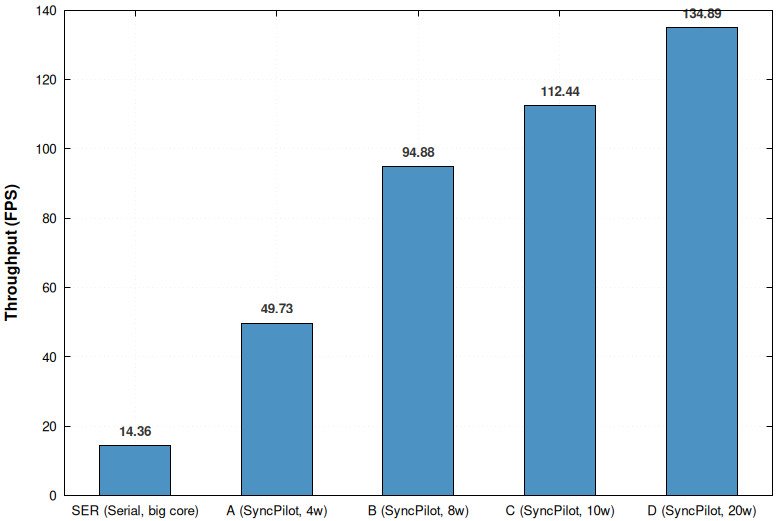
\includegraphics[width=0.85\columnwidth]{fsrcnn_throughput_asus.png}
\caption{Throughput comparison across all configurations. SyncPilot-20W achieves the highest throughput at 134.89 FPS.}
\label{fig:throughput}
\end{figure}

\begin{figure}[htbp]
\centering
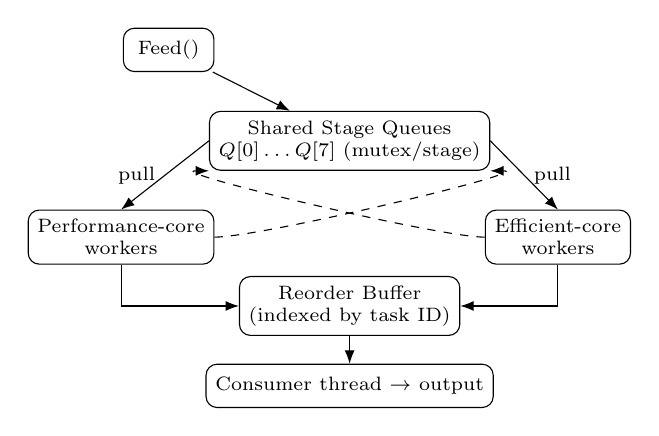
\begin{tikzpicture}[
    font=\scriptsize,
    box/.style={draw, rounded corners, minimum height=0.55cm, align=center},
    node distance=6pt
]
\node[box, minimum width=2.6cm] (q) {Shared Stage Queues\\$Q[0]\ldots Q[7]$ (mutex/stage)};
\node[box, minimum width=1.15cm, below left=14pt and -2pt of q] (big) {Performance-core\\workers};
\node[box, minimum width=1.15cm, below right=14pt and -2pt of q] (little) {Efficient-core\\workers};
\node[box, minimum width=2.6cm, below=14pt of q, yshift=-24pt] (rb) {Reorder Buffer\\(indexed by task ID)};
\node[box, minimum width=2.6cm, below=10pt of rb] (cons) {Consumer thread $\to$ output};
\node[box, minimum width=1.15cm, above left=14pt and -2pt of q] (feed) {Feed()};

\draw[-{Latex}] (feed) -- (q);
\draw[-{Latex}] (q.west) -- node[left]{pull} (big.north);
\draw[-{Latex}] (q.east) -- node[right]{pull} (little.north);
\draw[-{Latex}] (big) |- (rb.west);
\draw[-{Latex}] (little) |- (rb.east);
\draw[-{Latex}] (rb) -- (cons);
\draw[-{Latex}, dashed] (big.east) .. controls +(0.6,0) and +(0.6,0) .. (q.south east);
\draw[-{Latex}, dashed] (little.west) .. controls +(-0.6,0) and +(-0.6,0) .. (q.south west);
\end{tikzpicture}
\caption{SyncPilot pipeline engine. Performance- and Efficient-pinned workers pull tasks from a shared, priority-ordered set of per-stage queues (dashed arrows: push to the next stage) with no central dispatcher; the Reorder Buffer and consumer thread guarantee sequential output despite out-of-order completion.}
\label{fig:arch}
\end{figure}

\subsection{Calibration Overhead Analysis}
\label{sec:calibrationoverhead}
A key contribution of SyncPilot is the minimization of scheduling overhead through the IC-RCE mechanism. The calibration is performed only once during the first run (warm-up/profiling run). As shown in the benchmark data, the profiling run for SyncPilot-4W completed in 12342 ms. While this initial cost is higher than the serial baseline (10445 ms) due to cold-cache effects, thread initialization, and the overhead of invoking \texttt{clock\_gettime} for per-stage measurement, it is a strictly one-time penalty.

Once the Cost Table is populated, subsequent runs (Task ID $> 0$) operate in steady state with zero profiling overhead. The scheduling logic simply performs a lookup in the pre-calibrated table, consuming only a few CPU cycles per task dispatch. This contrasts sharply with continuous-monitoring approaches, where timing functions are invoked for every frame, accumulating measurable overhead over time and preventing the system from reaching optimal throughput.

\subsection{Per-Layer Execution Analysis: The IC-RCE Cost Table}
\label{sec:layerprofile}
The reference paper \cite{annisa2025fsrcnn} conducted a detailed per-layer execution time analysis, revealing that Layer 8 (deconvolution) dominates the computational cost across all configurations. Table~\ref{tab:layers} reports the IC-RCE Cost Table itself, i.e., the raw per-stage measurements produced by the calibration step described above, captured during the first-frame calibration pass on a Performance core.

\begin{table}[htbp]
\caption{IC-RCE Cost Table: Per-Layer Execution Time (Single-Frame Calibration Pass, Performance Core)}
\begin{center}
\small
\begin{adjustbox}{max width=\columnwidth}
\begin{tabular}{|l|c|c|c|}
\hline
\textbf{Layer} & \textbf{Stage} & \textbf{Time (s)} & \textbf{\% Total} \\
\hline
Layer 1 & Feature Extraction & 0.00562 & 6.0 \\
Layer 2 & Shrinking & 0.01389 & 14.7 \\
Layer 3 & Non-linear Mapping & 0.00654 & 6.9 \\
Layer 4 & Non-linear Mapping & 0.00365 & 3.9 \\
Layer 5 & Non-linear Mapping & 0.00322 & 3.4 \\
Layer 6 & Non-linear Mapping & 0.00327 & 3.5 \\
Layer 7 & Expanding & 0.01299 & 13.8 \\
Layer 8 & Deconvolution & 0.04514 & 47.9 \\
\hline
\textbf{Total} & & \textbf{0.09432} & \textbf{100.0} \\
\hline
\end{tabular}
\end{adjustbox}
\label{tab:layers}
\end{center}
\end{table}

Layer 8 (deconvolution, $9\times9$) dominates at 47.9\% of total per-frame calibration time (0.045~s out of 0.094~s), followed by Layer 2 (shrinking, $1\times1$) at 14.7\% and Layer 7 (expanding, $1\times1$) at 13.8\%. Together, Layers 7--8 account for 61.7\% of the per-frame cost, confirming the final stages as the primary computational bottleneck. This aligns with \cite{annisa2025fsrcnn}, where Layer 8 showed the lowest speedup across all parallel scenarios due to the $9\times9$ kernel requiring substantially more multiply-accumulate operations per output pixel.

Note that this single-frame calibration total (94.32~ms) is noticeably higher than the amortized steady-state per-frame cost implied by the serial baseline (10445~ms / 150~frames $\approx$ 69.6~ms/frame, Table~\ref{tab:throughput}) — a gap of roughly 35\%. This is expected rather than anomalous: the calibration pass is, by construction, the very first frame processed, before instruction and data caches are warm and while \texttt{clock\_gettime} is called around every stage boundary purely for measurement; both effects are one-time costs that IC-RCE is explicitly designed to tolerate (Section~\ref{sec:calibrationoverhead}) precisely because they occur only once. We do not have independent per-frame instrumentation of the steady-state serial run to confirm the 69.6~ms/frame figure directly (only its 150-frame aggregate); resolving this gap with fine-grained, per-frame timestamps is left as verification work.

When scaled across the full 150-frame sequence, Layer 8's dominance is consistent with the aggregate execution time distribution observed across configurations. This supports the IC-RCE assumption that computational costs are deterministic for a fixed input resolution, which is what makes a one-time, single-frame calibration a defensible substitute for continuous monitoring in this workload.

\subsection{Hardware Performance Counter Analysis}
\label{sec:perfcounter}
To further validate the efficiency of SyncPilot's design, we conducted hardware performance counter analysis using \texttt{perf stat}. 

Table \ref{tab:perf} presents the hardware performance counter analysis; the 1W and 2W columns are included only for trend continuity (Section~\ref{sec:setup}) and are not evaluated elsewhere in this paper. SyncPilot-4W and SyncPilot-8W maintain high instruction-level parallelism with IPC values of 3.60 and 3.64 respectively on the Cortex-X925 Performance cores. The cache miss rate remains low across worker configurations (1.95\% for 4W and 1.88\% for 8W), demonstrating efficient memory access patterns across pipeline stages.

The 20W row's IPC (2.97*) and instruction count (126,761~M, vs. $\approx$166,000~M for other configurations) are marked as measurement artifacts rather than as reliable per-instruction data; the mechanism is analyzed below using controlled experiments, not asserted from this table alone.

\begin{table}[htbp]
\caption{Hardware Performance Counter Comparison (perf stat)}
\begin{center}
\small
\begin{adjustbox}{max width=\columnwidth}
\begin{tabular}{|l|c|c|c|c|c|c|}
\hline
\textbf{Metric} & \textbf{1W (Serial)} & \textbf{2W} & \textbf{4W} & \textbf{8W} & \textbf{10W} & \textbf{20W} \\
\hline
IPC & 3.86 & 3.84 & 3.60 & 3.64 & 3.61 & 2.97* \\
CPI & 0.26 & 0.26 & 0.28 & 0.27 & 0.28 & 0.34 \\
Cache Ref (M) & 80,039 & 80,015 & 79,815 & 79,893 & 79,955 & 60,318 \\
Cache Miss (M) & 1,410 & 1,357 & 1,559 & 1,501 & 1,466 & 1,501 \\
Miss Rate (\%) & 1.76 & 1.70 & 1.95 & 1.88 & 1.83 & 2.49 \\
Cycles (M) & 43,217 & 43,406 & 46,291 & 45,845 & 46,250 & 42,728 \\
Instr (M) & 166,659 & 166,639 & 166,735 & 166,845 & 166,929 & 126,761* \\
\hline
\multicolumn{7}{l}{\footnotesize *PMU sampling coverage falls to 82--83\% at 20W (vs.\ 99.7\% at $\le$10W); see analysis below.}\\
\end{tabular}
\end{adjustbox}
\label{tab:perf}
\end{center}
\end{table}

Two hardware-level factors, isolated with the controlled experiments in Table~\ref{tab:ipcproof}, together explain the apparent IPC drop from 3.86 (1W) to 2.97 (20W, whole-system aggregate).

\textbf{PMU time-multiplexing artifact.} At 20 workers, the 20 highly active threads saturate the hardware PMU sampling budget, causing the kernel to time-multiplex event counting. Sampling coverage falls to 82--83\% vs. 99.7\% for configurations of 10W and below, causing the aggregate instruction count to appear at 126,761~M rather than the expected $\approx$166,000~M. Part of the reported drop in aggregate IPC is therefore a sampling artifact rather than a true per-instruction degradation; we do not, however, attribute the entire drop to this effect (see below).

\textbf{Efficient cluster activation.} The 20W configuration activates the Efficient core cluster (cluster~56, cpu0--9), which had contributed only 97~M instructions at 10W but contributes 72,379~M instructions at IPC~2.22 at 20W. Table~\ref{tab:ipcproof} reports two controlled runs isolating the Performance cluster's own counters: pinning 20 workers to Performance-cluster cores only (EXP-2) gives Performance-cluster IPC 2.95, and monitoring only the Performance-cluster counters while the full 20W (Performance+Efficient) configuration runs (EXP-4) gives 2.99 — not lower than EXP-2, which is the comparison that rules out cross-cluster L3 contention as a contributor. EXP-3 monitors the Efficient cluster in isolation during the same full 20W run and measures Efficient-cluster IPC at 2.22, substantially below the Performance cluster's own $\sim$3.6 IPC observed elsewhere in Table~\ref{tab:perf} at lower worker counts. It is this genuinely lower-IPC Efficient-cluster contribution being folded into the whole-system aggregate — not L3 interference, and only partly the PMU sampling artifact above — that pulls the reported 20W aggregate IPC down to 2.97.

\begin{table}[htbp]
\caption{Controlled IPC Experiments (ASUS GX10, 20 Workers)}
\begin{center}
\small
\begin{tabular}{|l|l|c|}
\hline
\textbf{Exp.} & \textbf{Configuration} & \textbf{IPC} \\
\hline
EXP-2 & 20W, pinned to Performance cluster only & 2.95 \\
EXP-3 & 20W (full run), Efficient cluster counters only & 2.22 \\
EXP-4 & 20W (full run), Performance cluster counters only & 2.99 \\
\hline
\end{tabular}
\label{tab:ipcproof}
\end{center}
\end{table}

\subsection{Function-Level Profiling Analysis}
\label{sec:gprof}
We performed function-level profiling using \texttt{gprof} to identify the computational hotspots in the FSRCNN pipeline. On Linux, \texttt{gprof}'s default sampling profiler only instruments the calling thread, so the self-time figures below characterize the main thread's call graph and are only a proxy for aggregate worker behavior; we report them as such rather than as a full multithreaded profile. The profiling results are nonetheless consistent with the layer-level cost distribution in Table \ref{tab:layers}, with the deconvolution functions dominating self time across all configurations.

\begin{table}[htbp]
\caption{Top Functions by Self Time (gprof Flat Profile, SyncPilot-10W)}
\begin{center}
\small
\begin{adjustbox}{max width=\columnwidth}
\begin{tabular}{|l|c|c|c|}
\hline
\textbf{Function} & \textbf{Self Time (s)} & \textbf{\% Total} & \textbf{Associated Layer} \\
\hline
deconv & 5.51 & 53.29 & Layer 8 (Deconvolution) \\
imfilter (L2/L3--6) & 1.39 & 13.44 & Layers 2, 3--6 \\
pad\_image & 0.76 & 7.35 & Layer support \\
imfilter (L1) & 0.67 & 6.48 & Layer 1 support \\
layer7 & 0.59 & 5.71 & Layer 7 (Expanding) \\
layer8 & 0.50 & 4.84 & Layer 8 (wrapper) \\
layer1--6 (combined) & 0.92 & 8.89 & Layers 1--6 \\
SyncPilot framework & 0.00 & 0.00 & Synchronization \\
\hline
\end{tabular}
\end{adjustbox}
\label{tab:gprof10w}
\end{center}
\end{table}

Table \ref{tab:gprof10w} presents the top functions by self time for SyncPilot-10W, the all-Performance-core configuration (10 workers pinned exclusively to the high-capacity cluster). The \texttt{deconv} function (Layer 8) dominates execution time, consistent with the per-layer analysis in Table \ref{tab:layers}. This dominance is attributed to the high multiply-accumulate count required for the upscaling operation (176$\times$144 $\rightarrow$ 352$\times$288) and the memory bandwidth demands of reading and writing large feature maps.

The SyncPilot framework functions register 0.00~s of \emph{main-thread} self time. Given \texttt{gprof}'s single-thread sampling limitation noted above, we read this as consistent with — but not proof of — low synchronization overhead on the sampled thread; it should not be read as a measurement of aggregate cross-thread synchronization cost, which would require a per-thread profiler such as \texttt{perf record}.

\begin{table}[htbp]
\caption{Top Functions by Self Time (gprof Flat Profile, SyncPilot-20W)}
\begin{center}
\small
\begin{adjustbox}{max width=\columnwidth}
\begin{tabular}{|l|c|c|c|}
\hline
\textbf{Function} & \textbf{Self Time (s)} & \textbf{\% Total} & \textbf{Associated Layer} \\
\hline
deconv & 4.74 & 51.97 & Layer 8 (Deconvolution) \\
imfilter (L2/L3--6) & 1.06 & 11.62 & Layers 2, 3--6 \\
pad\_image & 0.93 & 10.20 & Layer support \\
layer8 & 0.59 & 6.47 & Layer 8 (wrapper) \\
layer7 & 0.50 & 5.48 & Layer 7 (Expanding) \\
imfilter (L1) & 0.46 & 5.04 & Layer 1 support \\
layer1--6 (combined) & 0.83 & 9.10 & Layers 1--6 \\
main + overhead & 0.01 & 0.11 & - \\
SyncPilot framework & 0.00 & 0.00 & Synchronization \\
\hline
\end{tabular}
\end{adjustbox}
\label{tab:gprof20w}
\end{center}
\end{table}

Table \ref{tab:gprof20w} presents the gprof flat profile for SyncPilot-20W (self-time percentages computed against the table's own 9.12~s total). The \texttt{deconv} function (Layer 8) dominates at 51.97\% (4.74~s), consistent with the 10W result (Table \ref{tab:gprof10w}). Notably, the profile exposes two additional significant contributors that emerge at scale: \texttt{imfilter} variants (11.62\% + 5.04\%) and \texttt{pad\_image} (10.20\%), together accounting for 26.9\% of total time. These correspond to the image filtering and boundary padding operations within the convolution layers (Layers 1--6). At 20 workers, more threads concurrently execute these memory-intensive helper functions, amplifying their aggregate cost. As at 10W, the SyncPilot framework functions register 0.00~s of main-thread self-time; subject to the same single-thread-sampling caveat above, this is consistent with low overhead on the sampled thread but does not, on its own, establish that aggregate synchronization overhead is negligible at peak parallelism.

\subsection{Output Correctness Verification}
Output correctness was verified across all SyncPilot configurations and compared with the reference paper's findings. Every one of the 150 output frames in every scenario was bit-exact against the ground truth, confirmed by pixel-wise comparison (0 differing bytes) and infinite PSNR. We report this as an expected consequence of FSRCNN's deterministic arithmetic combined with the Reorder Buffer's sequencing guarantee, rather than as a surprising finding on its own; its value is as a direct contrast to \cite{annisa2025fsrcnn}, which reported that the Efficient CPU parallel scenario produced visible artifacts and pixel corruption due to race conditions during the deconvolution stage. SyncPilot's synchronized worker pool with reorder buffer rules out that class of race condition by construction, ensuring bit-exact outputs regardless of the worker configuration.

\subsection{Worker Configuration Analysis}
\label{sec:workerconfig}
The benchmark results reveal important insights about the optimal worker configuration for asymmetric pipeline processing.

Performance consistently improves as the worker count increases on ASUS GX10. SyncPilot-4W achieves a 3.46$\times$ speedup (3016 ms), SyncPilot-8W reaches 6.61$\times$ (1581 ms), SyncPilot-10W reaches 7.83$\times$ (1334 ms), and SyncPilot-20W achieves the best performance at 9.39$\times$ (1112 ms). This scaling behavior reflects the hardware characteristics of ASUS GX10: the Cortex-A725 Efficient cores are considerably stronger than older Efficient core implementations, so they do not become severe stragglers when assigned heavy stages. Consequently, SyncPilot can safely exploit additional parallelism without sacrificing the critical-path performance of the deconvolution stage. This finding extends the reference paper's result \cite{annisa2025fsrcnn}, where broader worker scaling across both Performance and Efficient cores delivered the strongest gains.

At 20 physical cores, a 9.39$\times$ speedup corresponds to approximately 47\% parallel efficiency, short of linear scaling; part of this is the expected consequence of pinning the two clusters at different clock/IPC operating points (Section~\ref{sec:perfcounter}), and part is queueing/reorder-buffer overhead that a purely embarrassingly-parallel scheme would not pay. This raises a fair question: with 150 independent frames, why not simply parallelize at the frame level (e.g., a \texttt{parallel for} over frames, each processed serially through all 8 layers) rather than an 8-stage pipeline? Frame-level parallelism would indeed be simpler and is plausibly at least as fast on this workload; we did not benchmark it directly, so we cannot claim the pipeline is faster. The stage-pipelined design is motivated instead by two structural requirements that a naive frame-level split does not address by itself: (1) bounded per-frame memory — pipelining constrains the number of frames in flight to \texttt{queue\_capacity\_per\_stage} per stage via backpressure, whereas naive frame-level parallelism holds one full set of intermediate feature maps per in-flight frame; and (2) it generalizes to streaming inputs where frames are not all available upfront (e.g., live video), for which a frame-level \texttt{parallel for} does not directly apply. A rigorous comparison against an optimized frame-level baseline is left as future work.

\subsection{CFS Baseline Comparison}
\label{sec:cfsidle}
As described in Section~\ref{sec:setup}, we additionally benchmarked a CFS baseline in which 10 and 20 threads are spawned without explicit CPU affinity, leaving thread-to-core placement entirely to the Linux Completely Fair Scheduler (CFS) with Energy Aware Scheduling (EAS) enabled on the ASUS GX10 kernel. This ablation isolates the specific contribution of SyncPilot's explicit Asymmetry-Aware Mapping relative to simply spawning an equivalent number of unpinned threads.\footnote{The CFS baseline was collected in a separate benchmark session from the headline results in Table \ref{tab:throughput}, following the same 8-run (1 warm-up + 7 averaged) protocol described in Section~\ref{sec:setup}. Consequently, SyncPilot-20W shows minor run-to-run variation between sessions (1112 ms in Table \ref{tab:throughput} vs. 1133 ms here), consistent with the low variance we observe across steady-state runs on this platform.}

\begin{table}[htbp]
\caption{SyncPilot vs. Unpinned CFS Baseline (Idle System)}
\begin{center}
\small
\begin{tabular}{|l|c|c|c|}
\hline
\textbf{Config.} & \textbf{Time (ms)} & \textbf{FPS} & \textbf{Speedup} \\
\hline
Serial (Performance Core) & 10452 & 14.35 & 1.00$\times$ \\
SyncPilot-10W & 1345 & 111.52 & 7.77$\times$ \\
CFS-10W (No Affinity) & 1343 & 111.69 & 7.78$\times$ \\
SyncPilot-20W & 1133 & 132.39 & 9.23$\times$ \\
CFS-20W (No Affinity) & 1046 & 143.40 & 9.99$\times$ \\
\hline
\end{tabular}
\label{tab:cfsbaseline}
\end{center}
\end{table}

Table \ref{tab:cfsbaseline} shows that, contrary to our initial expectation, unpinned CFS-20W outperforms SyncPilot-20W by 7.6\% on an idle system (1046 ms vs. 1133 ms), and the two approaches are statistically indistinguishable at 10 workers (1343 ms vs. 1345 ms). This result arises because on an idle ASUS GX10, Linux EAS is able to passively learn thread utilization patterns over the course of the 150-frame run and organically migrate compute-heavy threads toward Performance cores and light threads toward Efficient cores, converging toward a mapping similar to SyncPilot's explicit assignment, without incurring the fixed calibration or hard-pinning cost. Section~\ref{sec:noise} revisits this result under realistic system load, where the advantage of explicit semantic mapping becomes apparent.

% === VI. DISCUSSION ===
\section{Discussion}
\label{sec:discussion}

\subsection{Why Additional Workers Scale on ASUS GX10}
A counterintuitive but important finding is that on ASUS GX10, increasing the number of workers improves performance rather than degrading it. The 20-worker configuration achieves the best throughput at 1112 ms, while the 4-worker configuration trails at 3016 ms. This result reflects the hardware characteristics of ASUS GX10: the Cortex-A725 Efficient cores are considerably stronger than the Cortex-A55 cores used on the earlier platform, so they do not become severe stragglers when assigned heavy stages. Consequently, SyncPilot can safely exploit additional parallelism without sacrificing the critical-path performance of the deconvolution stage.

\subsection{System Noise Robustness: CFS/EAS vs. Static IC-RCE Mapping}
\label{sec:noise}
The idle-system result in Section~\ref{sec:cfsidle} raises a natural question: if unpinned CFS achieves higher raw throughput than SyncPilot's static mapping, what is the practical benefit of hard-pinning at all? We argue the answer lies in the difference between an idle benchmark environment and a real-world edge deployment, where the CPU concurrently services other workloads (e.g., network I/O, UI rendering, background daemons) rather than running FSRCNN in isolation. We consider this comparison, not the idle-system throughput numbers in Section~\ref{sec:cfsidle}, the central empirical result of this paper.

To evaluate this, we injected synthetic system noise using unpinned, CPU-bound OpenMP threads running alongside the FSRCNN-20W benchmark, and measured, for each of the 7 averaged runs per condition, the mean per-run latency and the worst (maximum) of the 7 per-run latencies. We refer to the latter as \emph{worst-case run latency} rather than "jitter" in the strict frame-to-frame sense, since our instrumentation records one wall-clock time per full 150-frame run, not a timestamp per frame; a genuine frame-level jitter characterization (per-frame latency distribution, p95/p99, standard deviation) would require finer-grained logging than we collected and is left as follow-up work (Section~\ref{sec:limitations}). Two noise intensities were tested: 4 background threads (moderate load) and 10 background threads (heavy load, saturating the Performance cluster); the noise threads themselves were left unpinned.

\begin{table}[htbp]
\caption{Latency Under System Noise (ASUS GX10)}
\begin{center}
\small
\begin{adjustbox}{max width=\columnwidth}
\begin{tabular}{|l|l|c|c|c|}
\hline
\textbf{Noise} & \textbf{Config.} & \textbf{Avg (ms)} & \textbf{Worst-Case Run (ms)} & \textbf{Speedup*} \\
\hline
\multirow{2}{*}{Idle} & SyncPilot-20W & 1133 & 1171 & 9.23$\times$ \\
 & CFS-20W & 1046 & 1067 & 9.99$\times$ \\
\hline
\multirow{2}{*}{4 Threads} & SyncPilot-20W & 1216 & 1256 & 8.60$\times$ \\
 & CFS-20W & 1314 & 1344 & 7.95$\times$ \\
\hline
\multirow{2}{*}{10 Threads} & SyncPilot-20W & 1402 & 1427 & 7.46$\times$ \\
 & CFS-20W & 1689 & 1769 & 6.19$\times$ \\
\hline
\multicolumn{5}{l}{\footnotesize *All speedups relative to the single 10452~ms idle serial baseline (Table~\ref{tab:cfsbaseline});}\\
\multicolumn{5}{l}{\footnotesize serial execution was not separately re-measured under noise.}\\
\end{tabular}
\end{adjustbox}
\label{tab:noise}
\end{center}
\end{table}

Table \ref{tab:noise} shows a reversal of the idle-system result. Under moderate noise (4 threads), SyncPilot-20W already overtakes CFS-20W in both average latency (1216 ms vs. 1314 ms) and worst-case run latency (1256 ms vs. 1344 ms). Under heavy noise (10 threads), the gap widens substantially in absolute terms: SyncPilot-20W's worst-case run latency grows from 1171 ms (idle) to 1427 ms, while CFS-20W's grows from 1067 ms (idle) to 1769 ms — SyncPilot remains faster in the worst case despite starting from a slower idle baseline. Expressed relative to each configuration's own idle baseline, this is a 21.9\% increase for SyncPilot-20W versus 65.8\% for CFS-20W; we report the absolute figures as the primary result and the relative growth only as a secondary, normalized view, since the relative framing alone could be read as inflating the comparison.

This behavior is consistent with the documented failure mode of Linux Energy Aware Scheduling (EAS). The kernel scheduler documentation states that once any CPU's utilization crosses the platform's overutilization threshold, EAS is disabled for the entire root domain and the generic, fairness-driven load balancer takes over for wake-up and load balancing \cite{linuxeas}. Under system noise, this is precisely what occurs on the Performance cluster: EAS's energy- and capacity-aware placement is deactivated, and CFS's fallback load balancer, which has no notion of which thread lies on the DNN's critical path, takes over. When background noise occupies the Performance cluster, this fallback balancer may migrate a pending Layer 8 (deconvolution) task to an Efficient core to preserve fairness, incurring a straggler penalty on the critical path. SyncPilot's hard-pinned static mapping (Section~\ref{sec:asymmap}) admits no such migration path: heavy stages remain on Performance cores and instead share CPU time with the noise via context switching, which raises average latency but bounds worst-case run latency far more tightly. We therefore conclude that SyncPilot's idle-system throughput deficit relative to unpinned CFS is offset by better latency stability under the non-idle conditions representative of real deployed edge devices; a full characterization of this trade-off under diverse, realistic background workloads, and with true per-frame jitter instrumentation, is left to future work.

\subsection{Race Condition Mitigation}
A significant finding from \cite{annisa2025fsrcnn} was that parallel FSRCNN execution on Efficient CPUs produced visible artifacts and pixel corruption due to race conditions during the deconvolution stage. Their serial execution produced artifact-free frames, while the parallel Efficient CPU scenario showed degraded image quality. In contrast, every SyncPilot configuration produced bit-exact outputs against the ground truth across all 150 frames (0 differing bytes; infinite PSNR). This improvement stems from SyncPilot's synchronized architecture: the pull-based worker pool with shared stage queues and reorder buffer ensures that each stage's output is correctly sequenced before being consumed by the next stage, structurally ruling out the race conditions that affected the reference paper's OpenMP-based parallelization.

\subsection{Scalability and Limitations}
\label{sec:limitations}
The current implementation of SyncPilot is optimized for steady-state workloads with fixed input characteristics. The IC-RCE mechanism assumes that the computational cost of each pipeline stage remains deterministic for a given input resolution. This assumption holds for FSRCNN with constant-resolution video streams (176$\times$144 $\rightarrow$ 352$\times$288), as confirmed by the low variance across steady-state runs. However, if the input workload changes drastically mid-stream (e.g., a resolution switch from 480p to 1080p), the initial calibration becomes invalid and a recalibration trigger would be required. Future work could integrate a lightweight anomaly detector to identify cost deviations and trigger a recalibration cycle, maintaining adaptability without sacrificing the low overhead of the steady-state phase.

Several further limitations should be stated explicitly. First, we do not report an ablation isolating IC-RCE's specific contribution from that of static core pinning: the GX10 results in this paper use capacity-agnostic, priority-ordered pulling (Section~\ref{sec:capacityaware}) throughout, so the reported numbers already reflect "pinning without cost-gated routing" rather than a pinning-plus-explicit-threshold-routing configuration; a controlled comparison against the framework's optional \texttt{enable\_two\_pool} cost-threshold-gated pulling mode, and against a continuously-monitored (non-calibrate-once) baseline, on this platform is left as future work rather than reported here. Second, the $0.75\times$ mean-cost threshold used by the optional cost-gated mode (Section~\ref{sec:capacityaware}) has not been swept or sensitivity-tested. Third, our noise experiment (Section~\ref{sec:noise}) uses unpinned background threads; a variant pinned specifically to the Performance cluster, representing a worst-case contention scenario, is not yet tested, nor have we tested a work-conserving fallback that would let idle Efficient workers assist with backlogged heavy stages under contention. Fourth, all claims of energy efficiency implied by "Efficient-core-friendly" scheduling in earlier sections of this paper are motivational rather than measured: we did not collect on-board power telemetry, and we do not report energy numbers; quantifying the energy trade-off of hard-pinning vs. CFS/EAS is left entirely to future work. Fifth, we do not release an artifact or code package alongside this submission; we intend to do so in a revision.

% === VII. CONCLUSION ===
\section{Conclusion}
We presented SyncPilot, a lightweight pipeline scheduling framework for asymmetric multicore architectures, built around Initial Calibration Runtime Cost Estimation (IC-RCE): a one-time, first-frame calibration that measures per-stage cost and empirically justifies relying on a static, hardware-topology-based Performance/Efficient core mapping rather than a continuously-monitored one. Our evaluation on ASUS GX10 using FSRCNN for low-to-high resolution video reconstruction (176$\times$144 $\rightarrow$ 352$\times$288, Suzie sequence) shows that SyncPilot-20W achieves a 9.39$\times$ speedup (134.89 FPS, 1.112~s) over the serial baseline (14.36 FPS, 10.445~s), at roughly 47\% parallel efficiency. The IC-RCE Cost Table confirms Layer 8 (deconvolution) as the dominant per-frame cost, consistent with prior findings on a more classically heterogeneous platform \cite{annisa2025fsrcnn}. Every configuration produced bit-exact outputs against the ground truth across all 150 frames, confirming that the framework maintains correctness while improving throughput. Notably, on an idle system the default CFS scheduler with Energy Aware Scheduling can match or even exceed SyncPilot's raw throughput, as it is able to passively learn a near-optimal thread-to-core mapping in the absence of competing workloads; however, under synthetic system noise representative of real, non-idle edge deployments, SyncPilot's hard-pinned static mapping yields both higher throughput and a substantially smaller worst-case latency increase than the unpinned CFS baseline, a direct consequence of CFS's Energy Aware Scheduling being disabled under CPU overutilization. We consider this noise-robustness result, rather than the idle-system throughput numbers, the paper's central finding: for edge AI workloads that must share the CPU with other processes, a cheap one-time calibration that licenses a fixed mapping can be a more reliable design choice than an OS scheduler that continuously re-optimizes but loses that reliability precisely when the system is busiest. Future work includes an ablation isolating IC-RCE's contribution from static pinning, true per-frame jitter instrumentation, on-board energy measurement, and dynamic recalibration triggers for variable-resolution workloads.

% === REFERENCES ===
\begin{thebibliography}{00}

\bibitem{wang2020pipeit}
S. Wang, G. Ananthanarayanan, Y. Zeng, N. Goel, A. Pathania, and T. Mitra, ``High-Throughput CNN Inference on Embedded ARM big.LITTLE Multicore Processors,'' \textit{IEEE Transactions on Computer-Aided Design of Integrated Circuits and Systems}, vol. 39, no. 10, pp. 2254--2267, Oct. 2020.

\bibitem{shi2016edge}
W. Shi, J. Cao, Q. Zhang, Y. Li, and L. Xu, ``Edge Computing: Vision and Challenges,'' \textit{IEEE Internet of Things Journal}, vol. 3, no. 5, pp. 637--646, 2016.

\bibitem{zhou2019edge}
Z. Zhou, X. Chen, E. Li, L. Zeng, K. Luo, and J. Zhang, ``Edge Intelligence: Paving the Last Mile of Artificial Intelligence With Edge Computing,'' \textit{Proceedings of the IEEE}, vol. 107, no. 8, pp. 1738--1762, 2019.

\bibitem{greenhalgh2011biglittle}
P. Greenhalgh, ``Big.LITTLE Processing with ARM Cortex\texttrademark-A15 \& Cortex-A7,'' ARM White Paper, Sept. 2011.

\bibitem{arm2013biglittle}
ARM Ltd., ``big.LITTLE Technology: The Future of Mobile,'' ARM White Paper.

\bibitem{koufaty2010bias}
D. Koufaty, D. Reddy, and S. Hahn, ``Bias Scheduling in Heterogeneous Multi-core Architectures,'' in \textit{Proc. 5th European Conference on Computer Systems (EuroSys)}, 2010, pp. 125--138, doi: 10.1145/1755913.1755928.

\bibitem{vancraeynest2012pie}
K. Van Craeynest, A. Jaleel, L. Eeckhout, P. Narvaez, and J. Emer, ``Scheduling Heterogeneous Multi-Cores through Performance Impact Estimation (PIE),'' in \textit{Proc. 39th Annual International Symposium on Computer Architecture (ISCA)}, 2012, pp. 213--224, doi: 10.1109/ISCA.2012.6237019.

\bibitem{saez2010comprehensive}
J. C. S\'{a}ez, M. Prieto, A. Fedorova, and S. Blagodurov, ``A Comprehensive Scheduler for Asymmetric Multicore Systems,'' in \textit{Proc. 5th European Conference on Computer Systems (EuroSys)}, 2010, pp. 139--152, doi: 10.1145/1755913.1755929.

\bibitem{man7pthreadaffinity}
The Linux man-pages project, ``pthread\_setaffinity\_np(3) --- Linux manual page.'' [Online]. Available: https://man7.org/linux/man-pages/man3/pthread\_setaffinity\_np.3.html

\bibitem{linuxeas}
The Linux Kernel documentation, ``Energy Aware Scheduling.'' [Online]. Available: https://docs.kernel.org/scheduler/sched-energy.html

\bibitem{dong2016fsrcnn}
C. Dong, C. C. Loy, and X. Tang, ``Accelerating the Super-Resolution Convolutional Neural Network,'' in \textit{Proc. European Conference on Computer Vision (ECCV)}, 2016, pp. 391--407.

\bibitem{wang2021asymo}
M. Wang, S. Ding, T. Cao, Y. Liu, and F. Xu, ``AsyMo: Scalable and Efficient Deep-Learning Inference on Asymmetric Mobile CPUs,'' in \textit{Proc. ACM MobiCom}, 2021.

\bibitem{yuan2025dynpipe}
Z. Yuan, X. Wang, Y. Nie, Y. Tao, Y. Li, Z. Shao, X. Liao, B. Li, and H. Jin, ``DynPipe: Toward Dynamic End-to-End Pipeline Parallelism for Interference-Aware DNN Training,'' \textit{IEEE Transactions on Parallel and Distributed Systems}, vol. 36, no. 11, pp. 2366--2382, 2025.

\bibitem{annisa2025fsrcnn}
A. Annisa and Adnan, ``Enhancing computational efficiency: Transitioning from serial to parallel programming for low-to-high resolution video reconstruction using FSRCNN on AMP architecture,'' in \textit{Proc. IEEE Int. Conf. Artificial Intelligence and Mechatronics Systems (AIMS)}, 2025, pp. 1--8, doi: 10.1109/AIMS66189.2025.11229650.

\bibitem{chronaki2017task} 
K. Chronaki, A. Rico, M. Casas, M. Moretó, R. M. Badia, E. Ayguadé, J. Labarta, and M. Valero, ``Task Scheduling Techniques for Asymmetric Multi-core Systems,'' \textit{IEEE Transactions on Parallel and Distributed Systems}, vol. 28, no. 7, pp. 2074--2087, 2017.

\bibitem{saad2026qlsa}
A. Saad, O. Abd el-Raouf, M. Hadhoud, and A. Kafafy, ``QLSA-MOEAD integration for precision task scheduling in heterogeneous computing environments,'' \textit{Scientific Reports}, vol. 16, art. 7194, 2026, doi: 10.1038/s41598-026-36916-1.

\end{thebibliography}

\end{document}